\documentclass[api,pof,pre,12pt,a4paper]{revtex4-1}     
\usepackage{bm}
\usepackage{natbib}
\usepackage{url}
\usepackage[intlimits]{amsmath}
\usepackage{graphicx}
\usepackage{fancyhdr}
\usepackage{amsfonts}
\usepackage{amssymb}
%\usepackage{pstricks}
%\usepackage{pst-coil}
%\usepackage{pst-plot}
\usepackage{hyperref}

\newtheorem{theorem}{Theorem}
\newtheorem{prob}{Problem}
\newenvironment{problem}[1]{\begin{prob} {\rm #1} \end{prob}}

%Nadir's Shortcuts
\newcommand{\beqn}{\begin{equation}}
\newcommand{\eeqn}{\end{equation}}
\newcommand{\beqa}{\begin{eqnarray}}
\newcommand{\eeqa}{\end{eqnarray}}
\newcommand{\beqanonum}{\begin{eqnarray*}}
\newcommand{\eeqanonum}{\end{eqnarray*}}
\newcommand{\beqnonum}{\begin{equation*}}
\newcommand{\eeqnonum}{\end{equation*}}
\newcommand{\jump}{\vspace{0.5cm}}
\newcommand{\bbf}{\begin{bf}}
\newcommand{\ebf}{\end{bf}}
%\newcommand{\eqnref}[1]{(\ref{#1})}
\newcommand{\defn}[1]{\begin{bf}\emph{#1}\end{bf}}
\newcommand{\reals}{\ensuremath{\mathbb{R}}}
\newcommand{\complex}{\ensuremath{\mathbb{C}}}
\newcommand{\integers}{\ensuremath{\mathbb{Z}}}
\newcommand{\half}{\ensuremath{\frac{1}{2}}}
\newcommand{\n}{\nonumber}
\renewcommand{\d}{\mathrm{d}}
\newcommand{\del}{\partial}
\newcommand{\dd}{\ensuremath{\, \mathrm{d}}}
\newcommand{\nint}[4]{\int_{#3}^{#4} {#1}\, \mathrm{d}{#2}}
\newcommand{\der}[2]{\frac{\d {#1}}{\d {#2}}}
\newcommand{\parder}[2]{\frac{\del {#1}}{\del {#2}}}
\newcommand{\funder}[2]{\frac{\delta {#1}}{\delta {#2}}}
\newcommand{\Lag}{\mathcal{L}}

\oddsidemargin  0.0in
\evensidemargin 0.0in
\textwidth      6.5in
\headheight     15pt
\topmargin      0.0in
\textheight=8.0in
%\setlength{\parindent}{0in}

\lhead{Spatially periodic forcing in SH35}
\chead{}
\rhead{Gandhi \& Knobloch}
%\lfoot{}
%\cfoot{}
%\rfoot{}


%Figures
\newcommand{\FIGcowboy}{
\begin{figure}[t]\center
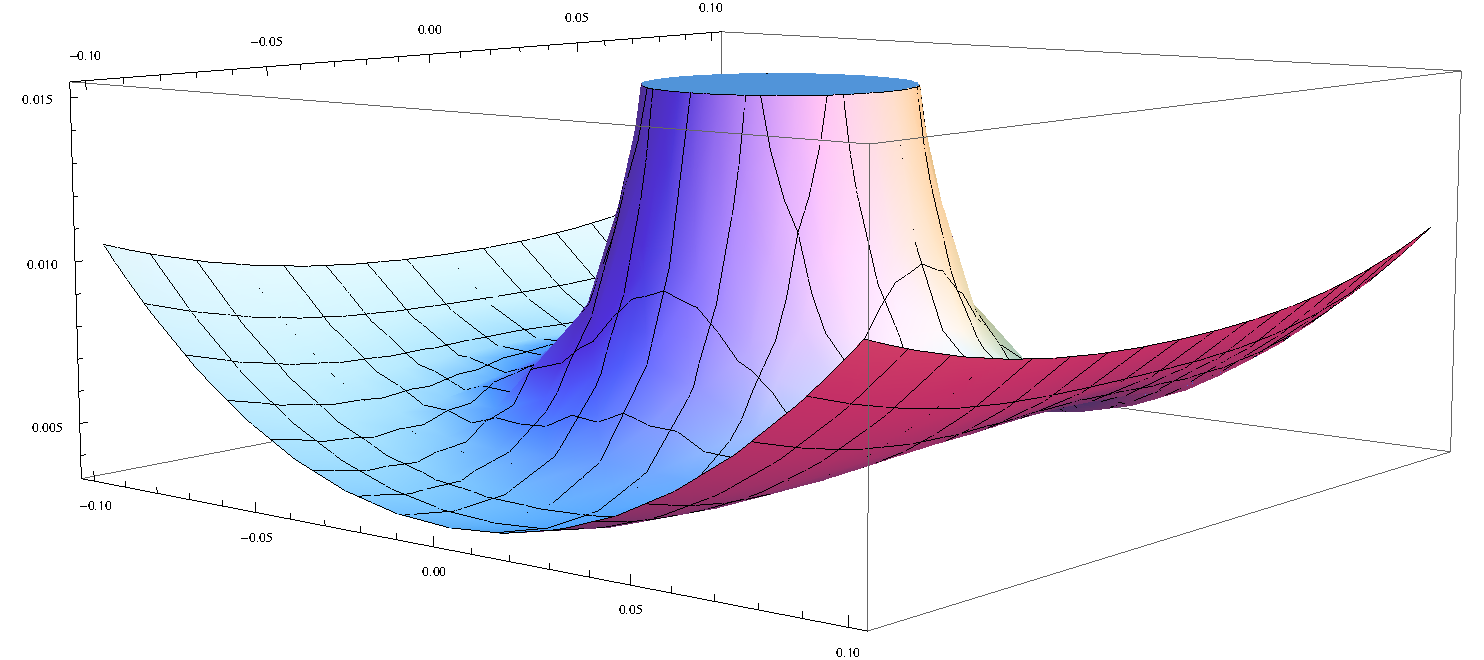
\includegraphics[width=60mm]{CowboyHatPotential.pdf}
\caption{\label{fig:CowboyHat} A plot of the cowboy hat potential with $l=0.005$, $\mu=1.0$, and $\gamma=0.5$.}
\end{figure}
}
\newcommand{\FIGforce}{
\begin{figure}[t]\center
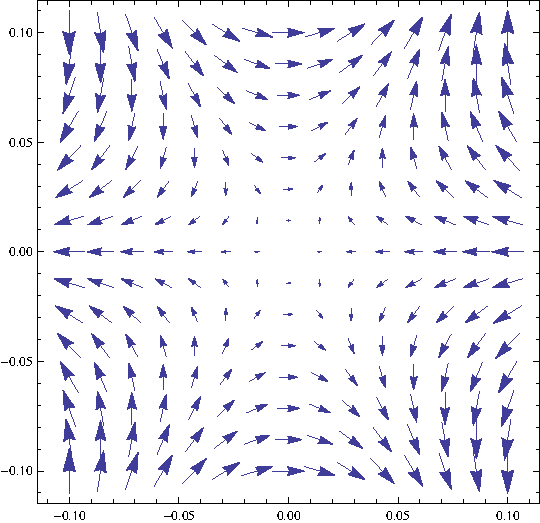
\includegraphics[width=60mm]{CowboyField.pdf}
\caption{\label{fig:CowboyForce} A plot of the force corresponding to the term of the potential that breaks radial symmetry.}
\end{figure}
}

\newcommand{\FIGorbits}{
\begin{figure}[t]\center
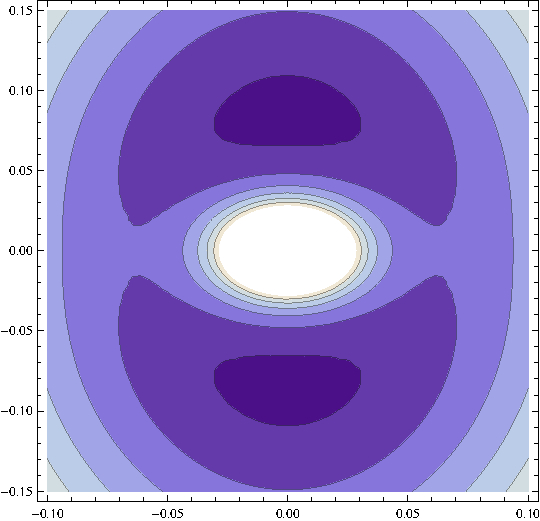
\includegraphics[width=60mm]{CowboyOrbits.pdf}
\caption{\label{fig:CowboyOrbits} A plot of the contours of $\bar{h}$ of Eq. \ref{eq:CowboyHat}. The darker color corresponds to lower energy.}
\end{figure}
}


\pagestyle{fancy}
\begin{document}
\preprint{APS/123-QED}

\title{Spatially periodic forcing in the Swift Hohenberg equation}

\author{Punit Gandhi}
 \email{punit_gandhi@berkeley.edu}
\author{Edgar Knobloch}
 \email{knobloch@berkeley.edu}
\affiliation{Department of Physics, University of California, Berkeley CA 94720, USA}

\begin{abstract}
We study the effect of a spatially periodic perturbation to the forcing term in the cubic-quintic Swift-Hohenberg equation (SH35).  We focus our analysis near the bifurcation point of the patterned state from the homogeneous state and develop an amplitude equation to describe the averaged dynamics at leading order.  
\end{abstract}

\maketitle

\section{Introduction}
The Swift-Hohenberg equation serves as a model for pattern formation in a broad range of physical systems.  We will be interested in the case of a cubic-quintic nonlinearity term, which allows for the existence of localized states.  This equation, which takes the form  
\begin{equation}
u_t= r u-\left(1+\partial_{x}^2\right)^2u+bu^3-u^5\label{eq:SH35},
\end{equation}
describes the dynamics of a real field $u$ over one spatial dimension in time.  We have rescaled the equation, which will be referred to as SH35, so that the critical wavenumber that defines the natural wavelength of the patterned state is unity. The strength of the linear forcing term $r$ and the strength of the quadratic nonlinearity $b$ are left as parameters of the system.  {\it (Some more details about work that has already been done on this equation)} 


Realistic systems will not always have a perfectly homogeneous forcing in space, and inhomogeneities may even lead to a way to manipulate dynamics of localized states. As a simple extension to Eq. \ref{eq:SH35}, we would now like to consider the case when the forcing has a periodic perturbation,
\begin{equation}
u_t= r(1+\delta \cos{\kappa x}) u -\left(1+\partial_{x}^2\right)^2u+bu^3-u^5\label{eq:SH35spf}.
\end{equation}

We can make some analytic progress on studying Eq.~\ref{eq:SH35spf} using techniques very similar to those used on the original equation (Eq.~\ref{eq:SH35}). We will look near the $r=0$ bifurcation point on a long timescale and a long spatial scale to get an amplitude equation at leading order.  In the special case that the periodicity of the forcing is half that of the natural wavelength, we obtain a parametrically forced Ginsburg-Landau equation for the amplitude.  


\section{Preliminary Analysis}
The addition of the periodic forcing perturbation does not destroy the variational structure of Eq. \ref{eq:SH35}.  Indeed, Eq. \ref{eq:SH35spf} can still be written in terms of a Lyapunov functional as 
\beqn
u_t=-\frac{\delta F}{\delta u},
\eeqn
where the Lyapunov functional F has been slightly modified
\beqn
F=\int -\frac{1}{2}r(1+\delta \cos\kappa x) u^2+\frac{1}{2}\left[(1+\partial_x^2) u\right]^2 -\frac{1}{4}bu^4+\frac{1}{6}u^6\; dx.
\eeqn
Therefore, we know that the system will still relax towards a steady state in time.  This motivates the study of time-independent solutions that will be pursued in following sections.

The trivial solution $u=0$ also still exists for the perturbed system (Eq. \ref{eq:SH35spf}). There can no longer be nonzero constant solutions as there were for certain parameter regimes of the original SH35.  To see this, we need only assume a constant solution for $u$ and we will run into  a contradiction when the constant is not zero (assume $\delta$ is nonzero).  


\section{Scaling}
We would like to look at small amplitude solutions in the neighborhood of the $r=0$ bifurcation where the periodic state branches off of the homogeneous state in the space of steady-state solutions.  We will take a multi-scale approach, defining a slow timescale $T=\epsilon^2t$, and long spatial scale $X=\epsilon x$ so that the derivatives become $\partial_t \rightarrow \partial_t+\epsilon^2\partial_T$ and $\partial_x \rightarrow \partial_x+\epsilon\partial_X$.  We will assume that the system will not change on the fast timescale, so we can neglect the $\partial_t$ term. With some trial and error, it can be seen that the appropriate scaling of forcing strength to probe the dynamics we are interested in will be $r=\epsilon^2 \mu$.     Additionally, we will not make any assumptions about $\delta$ yet, but will eventually want to consider the case that $\epsilon <<\delta <<1$.

With this scaling, Eq. \ref{eq:SH35spf} becomes 
\begin{equation}
\epsilon^2 u_T = \epsilon^2 \mu(1+\delta \cos{\kappa x}) u -\left(1+(\partial_{x}+\epsilon \partial_X)^2\right)^2u+bu^3-u^5
\label{eq:SH35spfeps}.
\end{equation}
Note we will also assume that the spatial periodicity of the forcing happens at a lengthscale comparable that of the characteristic wavelength of the patterned state.  In particular, we will focus on the case that $\kappa=2$, as this will lead a parametrically forced Ginzburg-Landau equation.

\section{Expansion}
We will write out the solution as an asymptotic expansion in the small parameter $\epsilon$:
\begin{equation}
u=\sum_{j=0}^{\infty} \epsilon^j u_j
\end{equation}
Since we want to look for small amplitude solutions, we will assume that $u_0=0$ and that the leading order solution comes in only at $\mathcal{O}(\epsilon)$. Furthermore, we can see by the structure of the nonlinear terms that we will not need the even powers of the expansion.  The equation that $u_2$ will need to satisfy, for example, will be identical to the one that $u_1$ will need to satisfy so that we could effectively redefine it by $u_1\rightarrow u_1+\epsilon u_2$.  We will finally note that the leading order effects of the spatially modulated forcing will by captured by making the expansion out to order $\mathcal{O}(\epsilon^3)$.   
\begin{equation}
u=\epsilon u_1 + \epsilon^3 u_3  + \mathcal{O}(\epsilon^5)
\label{eq:AsympExpU}
\end{equation}

We can now plug in the asymptotic series form of the solution Eq. \ref{eq:AsympExpU}) into the scaled version of the SHE35 (Eq. \ref{eq:SH35spfeps}) and match terms in orders of $\epsilon$.  The leading order terms will be $\mathcal{O}(\epsilon)$:
\begin{equation}
u_1+2\partial_x^2 u_1 +\partial_x^4 u_1 = 0.
\end{equation}
This equation has a solution of the form
\begin{equation}
u_1(x,X,T)=A(X,T) e^{i x}+ \bar{A}(X,T) e^{-ix},
\label{eq:u1sol}
\end{equation}
where $A(X,T)$ is a still undetermined complex amplitude that depends only on the slow timescale $T$ and the long lengthscale $X$, and $\bar{A}(X,T)$ is its complex conjugate. Collecting terms at the next order in $\epsilon$ will provide a solvability condition that we will use to determine $A$.

We can now go on to look at the next terms in the expansion, which come in at $\mathcal{O}(\epsilon^3)$:
\begin{eqnarray}
u_3+2\partial_x^2 u_3 &+& \partial_x^4 u_3 =  \nonumber \\
& & -\partial_T u_1-2\partial_X^2 u_1 - 6\partial_x^2 \partial_X^2 u_1 +\mu u_1 +\mu \delta \cos(\kappa x)  u_1 +b u_1^3
\label{eq:AsympExpEps3}
\end{eqnarray}
Plugging in the form of the solution for $u_1$ from Eq. \ref{eq:u1sol} gives the following expression for the RHS of the equation above.
\begin{eqnarray}
\text{RHS}&=&  \nonumber \\ 
& &\left(-A_T  +4 A_{XX}+\mu A + 3b |A|^2 A\right)e^{ix} + \left(-\bar{A}_T +4 \bar{A}_{XX}+\mu \bar{A} + 3b |A|^2 \bar{A}\right)e^{-ix} \nonumber \\
& &+\frac{\mu\delta}{2} A\left(e^{i(1+\kappa)x}+e^{i(1-\kappa)x} \right) + \frac{\mu\delta}{2} \bar{A}\left( e^{-i(1+\kappa)x}+e^{-i(1-\kappa)x} \right) \nonumber \\
& & +bA^3e^{3ix}+b\bar{A}^3e^{-3ix}
\label{eq:RHSeps3}
\end{eqnarray}
The resonant terms of in the above expression (Eq. \ref{eq:RHSeps3}) must vanish in order for this equation to be solved, giving the desired equation that determines the complex amplitude $A$.  The choice of $\kappa$ determines if the effects of the spatially periodic forcing perturbation can be seen at this order.  In particular, the choice of $\kappa=2$, modifies the complex amplitude equation so that it includes a parametric forcing term (proportional to $\bar{A}$).

\section{The 2:1 resonance in the forcing}
We will now focus on the case that the period of the forcing perturbation is half that of the characteristic wavelength of the patterned state, namely that $\kappa=2$.  Plugging this into Eq. \ref{eq:AsympExpEps3} leads to the following equation for the complex amplitude from the solvability condition that resonant terms vanish:
\begin{equation}
-A_T  +4 A_{XX}+\mu A + 3b |A|^2 A+\frac{\mu\delta}{2}\bar{A}=0
\label{eq:LGEpf1}
\end{equation}

With appropriate redefinitions of variables, we can put this equation into the following form
\begin{equation}
A_T  = \mu A + A_{XX} - |A|^2 A+\gamma\bar{A}
\label{eq:LGEpf}
\end{equation}
where we have assumed that $b<0$.

\subsection{Polar Coordinates}
Equation \ref{eq:LGEpf}  can now be put into a form that resembles a particle orbiting in central potential by making the substitution $A=r e^{i\theta}$, where $r$ and $\theta$ are real functions of $X$ and $T$.  The resulting pair of real pde's is:
\begin{subequations}
\begin{align}
\dot{r}&=\mu r - r^3 +r''-r\theta'^2+\gamma r \cos2\theta 
\label{eq:PolarGLEpfr} \\
r^2\dot{\theta}&=2 r r' \theta'+r^2\theta''-\gamma r^2 \sin 2\theta
\label{eq:PolarGLEpfth}
\end{align}
\end{subequations}
where the dot and prime represent derivatives with respect to the time $T$ and the position $X$, respectively.

\subsection{Constant amplitude solutions}
The original SH35 has periodic solutions that are time-independent and have a constant amplitude in space.  We can try to look for similar solutions to this case by assuming $r=r_0$ is a nonzero constant. Substituting this into Eq. \ref{eq:PolarGLEpfr} leads to
\beqn
\theta'^2=\mu-r_0^2+\gamma \cos2\theta
\label{eq:r0Polar1}
\eeqn
which,upon taking a derivate, gives
\beqn
\theta''=-\gamma \sin2\theta
\eeqn
On the other hand, Eq. \ref{eq:PolarGLEpfth} reduces to 
\beqn
\theta''=\gamma \sin2\theta
\eeqn
after making the constant amplitude assumption.  The only way for both of these equations to be true, assuming a nonzero $\gamma$, is for $\sin2\theta=0$. This implies that $\theta=n\pi/2$ must be constant, where $n$ is some integer.  Plugging value this of $\theta$ back into Eq. \ref{eq:r0Polar1} gives the corresponding possible values of the amplitude, $r_0=\sqrt{\mu +(-1)^n\gamma}$. Note that we only consider positive values of $r$ since a negative value corresponds to a $\pi$ shift in $\theta$. These solutions will exist in the parameter regime where $\mu\pm\gamma\ge 0$.  These constant solutions are straightforward to find from the original amplitude equation (Eq. \ref{eq:LGEpf}).  It is not difficult to see that the solutions $A=\pm i \sqrt{\mu-\gamma}$ are stable in space when they exist (i.e. $\mu \geq \gamma$), and the solutions $A=\pm \sqrt{\mu+\gamma}$ are unstable in space when they exist (i.e. $\mu \geq-\gamma$).


The solutions found here are constant in space and time for the amplitude, which correspond to periodic solutions to the perturbed SH35 (Eq. \ref{eq:SH35spf}). Explicitly, the leading order solutions are 
\beqn
u_1=\pm \frac{\sqrt{\mu-\gamma}}{2} \sin x,\: \pm \frac{\sqrt{\mu+\gamma}}{2} \cos x
\eeqn
{\it Should I go back and do this using the original amplitude equation I got from the perturbed SHE35 instead of the scaled version that is the CGLE?}
The $\sin$ solutions are stable in space and the $\cos$ solutions are unstable in space, but we need to go back and look at their stability in time.



\subsection{Time-independent solutions and spatial dynamics}
If we look for steady state solutions in time, we can reduce this problem to an ode with the dependent variable as space instead of time.  We can define a spatial {\it energy} $h$ and {\it angular momentum} $l$ by:
\begin{eqnarray}
l &=& r^2\theta' \\
h &=& \frac{1}{2} r'^2 +\frac{l^2}{2r^2} +\frac{1}{2}\mu r^2 -\frac{1}{4} r^4
\end{eqnarray}
In the limit that $\gamma$ vanishes, these new variables are actually constants of motion of the amplitude Eq. \ref{eq:LGEpf}.  The problem described by Eq. \eqref{eq:PolarGLEpfr} and \eqref{eq:PolarGLEpfth} can be mapped onto the problem of a particle traveling in a central potential equivalent to a particle in a central potential if we consider dynamics in space instead of time.  The spatial energy $h$ has a kinetic term, a effective potential term from the spatial angular momentum $l$, and a central potential well term.  Equations \eqref{eq:PolarGLEpfr} and \eqref{eq:PolarGLEpfth} can now be rewritten in terms of the spatial energy and angular momentum as:
\begin{subequations}
\begin{align}
l' &= \gamma r^2 \sin 2\theta 
\label{eq:CentPotL} \\
h'&= \gamma l \sin 2\theta-\gamma r r' \cos 2\theta
\label{eq:CentPotH}
\end{align}
\end{subequations}

Assuming $\epsilon <<\gamma <<1$ allows us to treat $l$ and $h$ as slowly varying quantities.  We could, in principle, apply the method of averaging to this equation to get spatially averaged equations that depend only on $l$ and $h$.  We would assume that these two quantities are constant and integrate over one period to average out the small variations of $r$ and $\theta$.  Unfortunately, this involves integrals that I'm not exactly sure how to do.

We can use the interpretation of a particle in a central potential to help us find solutions to our original problem that are localized in space and steady-state in time.  These type of solutions correspond to  orbits of the particle that approach $r=0$ as $x\rightarrow \pm \infty$.  We could look for these kinds of solutions to the unperturbed problem (when $\gamma=0$) and then try to understand what the perturbation does to these solutions. 

We can further simplify the energy equation by noting that the RHS is the spatial derivative of the quantity $-\half \gamma r^2 \cos 2 \theta$. By redefining the energy as
\beqn
\bar{h}=\frac{1}{2} r'^2 +\frac{l^2}{2r^2} +\frac{1}{2}\mu r^2 -\frac{1}{4} r^4+\half \gamma r^2 \cos 2 \theta,
\label{eq:CowboyHat}
\eeqn
so that the potential is no longer radially symmetric.  A plot of this potential, which will be referred to as the {\it cowboy hat potential}, is shown in Fig. \ref{fig:CowboyHat}.
\FIGcowboy
The force corresponding the additional energy term is $\mathbf{F}=-\gamma r (\cos2\theta \;\hat{r} - \sin2\theta \; \hat{\theta})$ is plotted in Fig. \ref{fig:CowboyForce}.    
\FIGforce
We can aslo plot contours of the modified energy (Eq. \ref{eq:CowboyHat}) to represent the orbits in the complex $A$ space. (Fig. \ref{fig:CowboyOrbits}).
\FIGorbits

\section{Future Work}
All of this works seems very straightforward, so I assume it must have been done somewhere. I've found a few things on the parametrically forced Complex Ginzbur-Landau equation that are related, but I can't seem to find this in the literature.  I need to keep looking. 

The next thing to do might be to look for localized solutions by looking for parameter regimes where it is possible for the orbit to approach 0 as $x \rightarrow \pm \infty$.  We would need to assume $l=0$ for this to be possible.

Another interesting thing to do might be to set up a time-stepping code for the SH35 with the periodic forcing and then see how one of these constant solutions that is stable for the amplitude equation evolves.  It might also be interesting to see how the trivial solution with some noise evolves in the parameter regime where it is unstable.  

One other thing I'd be interested in, is to see what happens if the forcing is slightly off from the 2:1 resonance. 
    



\bibliography{SpatialForcingBib}
\end{document}




